\chapter{Eigen Values problem}
We can now implement the eigenvalues problem from chapter \ref{eigen} to find the eigenpairs $(\lambda_i,\mathbf{g_i})$ such that $\curl\mathbf{g_i}=\lambda_i\mathbf{g_i}$ for $i=1,\dots,M$. Those functions will be the basis on which we will project $\mbf{u}$ for the Galerkin decomposition \[ \mathbf{u}=\sum_{i=1}^M c_i\mathbf{g_i} \]

\section{Discretization}
From now on, we'll use the following notations :
\begin{align*}
&\TT_h\mbox{ the set of tetrahedra } T \mbox{ such that }
\mbox{ such that } \Omega=\cup_{T\in\TT}T\\
&\TT_h^\Gamma =\{F\mbox{ faces of } T\in \TT_h \,|\, F\subset \Gamma
\}\\
&\NN^k(T)=[\PP_{k-1}(T)]^3\oplus\{\mbf{p}\in[\PP_k(T)]^3 \,|\,
\mbf{p(x)}\cdot\mbf{x}=0 \}\\
&\NN_h=\{\mbf{v}_h\in H(\mathrm{curl};\Omega) \,|\,
\mbf{v}_h\restr{T}\in\NN^k(T)\, \forall T\in \TT_h \}\\
&\ZZ_h=\NN_h\cap\ZZ=\{\mbf{v}_h\in\NN_h \,|\,
\curl\mbf{v}_h\cdot\mbf{n} = 0 \}
\end{align*}

The Galerkin approximation of Problem \ref{pbweak} reads :
\begin{pb}\label{pbdiscr}
Find $\lambda_h\in\CC$ and $\mbf{u}_h\in\ZZ_h$, $\mbf{u}_h\ne
0$, such that
\[\int_\Omega \curl\mbf{u}_h\cdot\curl\mbf{v}_h =
\lambda_h^2\int_\Omega \mbf{u}_h\cdot\mbf{v}_h \quad\quad
\forall\mbf{v}_h\in\ZZ_h \]
\end{pb}

The issue is to impose the condition
$\curl\mbf{u}_h\cdot\mbf{n}=0$ on $\Gamma$. Before, we tried to apply this
condition by a penalization method. But this was difficult, because we had to
find the proper parameter.\\

\subsection{A new basis}
\label{base}
In \cite{Venegas2013}, using \ref{relation} and following the method used in
\cite{Meddahi2003,Salgado2005}, they propose a basis to the space $\ZZ_h$.
Since it is based on the work of A. Buffa in \cite{Buffa2002845}, we need to
define some operators before we go on.
\begin{align*}
\pi_\tau(u) &= \mbf{n}\times\mbf{u}\times\mbf{n}\restr{\Gamma} &\mbox{the projection on
  the tangential plane}\\
\gamma_\tau(u) &= \mbf{u}\times\mbf{n}\restr{\Gamma} &\mbox{the tangential
  trace}\\
\grad_\Gamma(\varphi) &= \pi_\tau(\grad\varphi) &\mbox{the tangential gradient}\\
\mathrm{curl}_\Gamma(\varphi) &= \gamma_\tau(\grad\varphi) &\mbox{the tangential curl}
\end{align*}

Then, we have the equivalence :
\[ \curl\mbf{u}_h\cdot\mbf{n}=0\mbox{ on }\Gamma \iff
\mathrm{curl}_\Gamma(\pi_\tau(\mbf{u}_h))=0\quad \mbox{ on } \Gamma \]
and since $\mathrm{Ker(curl}_\Gamma)=\grad_\Gamma H^1(\Gamma)$ we have 
\[ \curl\mbf{u}_h\cdot\mbf{n}=0\mbox{ on }\Gamma \iff
\exists\varphi_h\in H^1(\Gamma) \mbox{ such that
}\mbf{n}\times\mbf{u}_h\times\mbf{n} = \grad_\Gamma\varphi_h \]
In fact, by \cite{Monk2003} Remark 5.29, we know that 
\[\varphi_h\in\LLL_h^\Gamma = \{\psi_h\in\mathcal{C}(\Gamma) \,|\,
\psi_h\restr{\Gamma}\in\PP_k(F) \quad \forall F\in\TT_h^\Gamma \}\]
the set of continuous functions which are piecewise polynomial on the faces of
the boundary.\\

The idea for creating the basis of $\ZZ_h$ is to take the basis of $\NN_h$, keep
only the functions define on the internal elements of the mesh and replace the
elements of the boundary by a basis of $\LLL_h^\Gamma$.\\

Let \[ \LLL_h=\{\psi\in\mathcal{C}(\Omega) \,|\,
\phi\restr{T}\in\PP_k(T)\,\forall T\in\TT_h^\} \]
and $\{\varphi_j\}_{j=1}^K$ be the nodal basis of $\LLL_h$.\\
We assume that the first J of them correspond to all the nodal values on the
boundary $\Gamma$. Then $\{\varphi_j\restr{\Gamma}\}_{j=1}^J$ is a
basis of $\LLL_h^\Gamma$ and
$\left\langle\{\grad_\Gamma\varphi_j\}_{j=1}^J\right\rangle=\grad_\Gamma(\LLL_h^\Gamma)$.\\
In order to have a basis, we have to choose one vertex on each connected
compoenent $\Gamma_0,\dots,\Gamma_I$ and remove the basis functions
corresponding. Assume that those functions are the last ones, then if
$L=J-(I+1)$, $\{\grad_\Gamma\varphi_j\}_{j=1}^L$ is a basis of
$\grad_\Gamma(\LLL_h^\Gamma)$.\\
Let $\{\bm{\phi}_m\}_{m=1}^M$ be the basis of $\NN_h$, where the last ones
correspond to the degrees of freedom related to the faces or edges on
$\Gamma$. We have that $\{\bm{\phi}_m\}_{m=1}^N$ lie in $\ZZ_h$.\\

Then the set $\{\bm{\phi}_m\}_{m=1}^N\cup  \{\grad\varphi_j\}_{j=1}^L$
is a basis of $\ZZ_h$.

\subsection{An algebraic solution}
In the case of the lowest order Nedelec elements, there is a way to impose the
condition $\curl\mbf{u}_h\cdot\mbf{n}=0$ without computing the basis seen in
  \ref{base}.\\
In the case of the lowest order, the degrees of freedom of the Nedelec elements
are \[\alpha_m=\int_{e_m} \mbf{u}_h\cdot\mbf{t}_m \quad m=1,\dots,M\] where $\{e_1,\dots,e_M\}$ is the set
of all edges in $\TT_h$ and $\mbf{t}_m$ is a unit vector tangent to $e_m$. The
direction of this vector depends on ...\\
Then we have \[\mbf{u}_h = \sum_{m=1}^M \alpha_m\bm{\phi}_m\]

Let $\{P_j\}_{j=1}^J$ be the set of vertices of $\TT_h^\Gamma$, and
$\{\varphi_j\}_{j=1}^J$ be the basis of $\LLL_h^\Gamma$, where the last $I$
functions are choses on a different connected component of $\Gamma$. Then, we have also :
\[ \mbf{u}_h = \sum_{m=1}^N \alpha_m'\bm{\phi}_m + \sum_{j=1}^L
\beta_j\grad\varphi_j \]
By identification, we obtain :
\[
\alpha_m=\left\{\begin{aligned}
&\alpha_m', &&\mbox{if } e_m\cap\Gamma = \emptyset, &\texttt{internalelements}\\
&\alpha_m'\pm \beta_j, &&\mbox{if } e_m\cap\Gamma = \{P_j\},& \texttt{boundaryelements}\setminus\texttt{boundaryedges}\\
&\alpha_m'\pm (\beta_j-\beta_k), &&\mbox{if } e_m\cap\Gamma = \{P_j,P_k\}
(e_m\notin\Gamma),& \texttt{boundaryelements}\setminus\texttt{boundaryedges}\\
&\pm (\beta_j-\beta_k), &&\mbox{if } e_m=[P_j,P_k]\subset\Gamma & \texttt{boundaryedges}
\end{aligned}\right.
\]
the signs depend on the direction of $t_m$.\\

We note $\bm{\alpha}=(\alpha_1,\dots,\alpha_M)^t$ and
$\widehat{\bm{\alpha}}=(\alpha_1',\dots,\alpha_M',\beta_1,\dots,\beta_J)^t$ and
then we can define a matrix $\mbf{C}\in\R^{M\times(N+L)}$ such that $\bm{\alpha}=\mbf{C}\widehat{\bm{\alpha}}$.\\

Let $\mbf{A}=(A_{ij})$ and $\mbf{B}=(B_{ij})$ be the $M\times M$ matrices defined
by 
\[A_{ij}=\int_\Omega \curl\bm{\phi}_j\cdot\curl\bm{\phi}_i \quad\mbox{and}\quad
B_{ij}=\int_\Omega\bm{\phi}_j\cdot\bm{\phi}_i\quad i,j=1,\dots,M \]
Then, by changing the basis, we have the following matrix form of Problem
\ref{pbdiscr} :
\begin{pb}\label{pbmat}
Find $\lambda_h\in\R$ and $\widehat{\bm{\alpha}}\in\R^{N+L}$ such that
\[ \widehat{\mbf{A}}\widehat{\bm{\alpha}} =
\lambda_h^2\widehat{\mbf{B}}\widehat{\bm{\alpha}} \]
where $\widehat{\mbf{A}}=\mbf{C}^t\mbf{A}\mbf{C}$ and $\widehat{\mbf{B}}=\mbf{C}^t\mbf{B}\mbf{C}$
\end{pb}

\section{Implementation}
\subsection{Details}

For the implementation of this problem, we need several steps :
\begin{itemize}
\item
  create the space $\mathbb{X}_h=\NN_hx\LLL_h$, we can do it using :
  \lstinputlisting[widthgobble=1*2,linerange={Xh}]{../../src/basischange.cpp}
\item
  create the matrix $A$ and $B$ :
  \lstinputlisting[widthgobble=1*2,linerange=forms]{../../src/basischange.cpp}
  The figure \ref{spyA} shows the sparsity pattern of $A$ : 
  \begin{figure}[H]
    \centering
    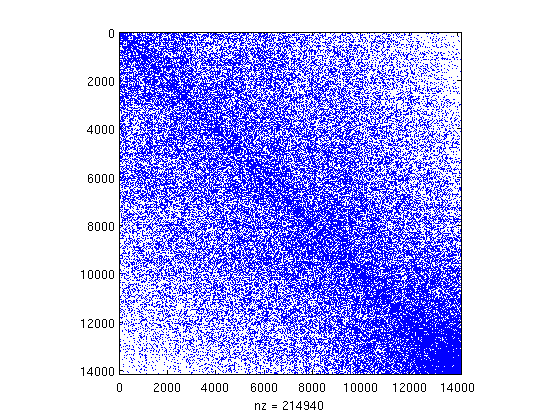
\includegraphics[scale=0.65]{spyA}
    \caption{Sparsity pattern of $A$}
    \label{spyA}
  \end{figure}
\item
  we can now use the function spaces previously defined to retrieve the
  informations on the dofs, if they are on the boundary or if they touch it.\\
  \begin{itemize}
  \item
    We first loop over all the degrees of freedom of $\NN_h$,
    \lstinputlisting[widthgobble=1*2,linerange=loop]{../../src/basischange.cpp}
  \item
    for all these dofs, we retrieve the edge associated and the permutation applied on this edge for the given element, if the permutation is the identity, the sign for the start of the edge is $-1$, else it is $+1$. The sign for the ending point of the edge is the opposite.
    \lstinputlisting[widthgobble=3*2,linerange=perm]{../../src/basischange.cpp}
  \item
    we now search for the dofs of $\LLL_h$ associated with these vertices. For this, we need to find the starting and ending points of the edge, relatively to the elements.\\
    This was the point where we were wrong before.
    \lstinputlisting[widthgobble=3*2,linerange=points]{../../src/basischange.cpp}
    Once we have the find the points, we need to find the corresponding dofs in $\LLL_h$
    \lstinputlisting[widthgobble=3*2,linerange=dofLh]{../../src/basischange.cpp}
  \item
    if the edge is on the boundary,
    \begin{itemize}
    \item
      we set its type,
    \item
      keep the two dofs of $\LLL_h$ corresponding to the vertices in memory,
    \item
      and keep the index of these dofs for later,
    \end{itemize}
  \item
    if the edge is not on the boundary,
    \begin{itemize}
    \item
      we keep the index of the dof for later,
    \item
      and if the two vertices are on the boundary, we set its type such that we
      know that it is {\bf not} on the boundary but it touches it with the two
      vertices, and we also keep the two dofs of $\LLL_h$,
    \item
      if only one vertex is on the boundary, we set its type accordingly, and
      keep the dof concerned,
    \item
      if the edge doesn't touch the boundary, we set its type to remember that.
    \end{itemize}
  \end{itemize}
\item
  We have the informations needed to construct a spanning set of $\ZZ_h$ but in order to have a basis, we have to remove one function, corresponding to a degree of freedom on the boundary. And that for each connected component of the boundary.\\
  For now, we handle only the case where there is just one component and at least one dof of it is on the first proc. 
  \lstinputlisting[linerange=remove]{../../src/basischange.cpp}
\item
  we now create the matrix $\tilde{C}$ of size $M\times (M+K)$. Using the informations retrieved on the dofs, we can now fill these two matrices :\\
  For each line of the two matrices,
  \begin{itemize}
  \item
    we set the first matrix to be the identity,
  \item
    if the edge touch the boundary with two vertices, we set the columns of
    the second matrix using the indexes of the two dofs corresponding to the
    vertices of the edge,
  \item
    if the edge touch the boundary with only one vertices, the start or the end of the edge, we set only the
    corresponding column,
  \item
    if the edge doesn't touch the boundary, these line stays empty. 
  \end{itemize}
  \lstinputlisting[linerange=fill]{../../src/basischange.cpp}
  The figure \ref{spyCTilde} shows the sparsity pattern of $\tilde{C}$ : 
  \begin{figure}[H]
    \centering
    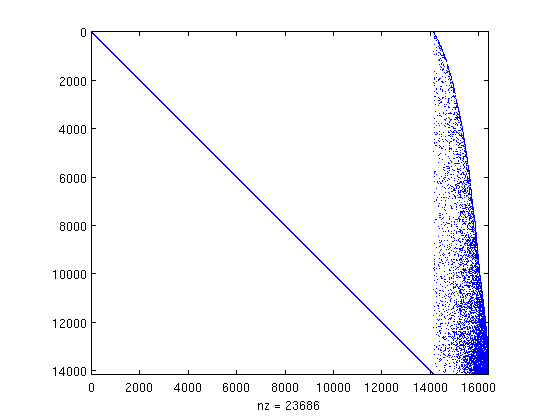
\includegraphics[scale=0.65]{spyCTilde}
    \caption{Sparsity pattern of $\tilde{C}$}
    \label{spyCTilde}
  \end{figure}
\item
  when we retrieved the informations on the dofs, we keep the indexes of the dofs of $\NN_h$ which {\bf are not} on the boundary and the indexes of the dofs of $\LLL_h$ which {\bf are} on the boundary. We only keep the columns of the matrix corresponding to these indexes.
  \lstinputlisting[widthgobble=1*2,linerange=submatrix]{../../src/basischange.cpp}
  The figure \ref{spyC} shows the sparsity pattern of $\tilde{C}$ : 
  \begin{figure}[H]
    \centering
    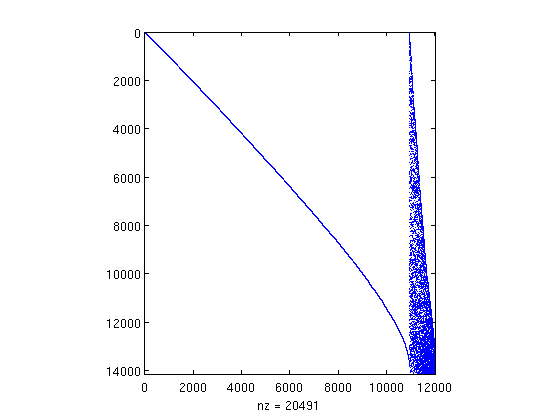
\includegraphics[scale=0.65]{spyC}
    \caption{Sparsity pattern of $C$}
    \label{spyC}
  \end{figure}
\item
  finally, create $\widehat{A}$ and $\widehat{B}$. We use for this the operator \texttt{PtAP} :
  \lstinputlisting[widthgobble=2*2,linerange=ptap]{../../src/basischange.cpp}
  The figure \ref{spyAA} shows the sparsity pattern of $\widehat{A}$ : 
  \begin{figure}[H]
    \centering
    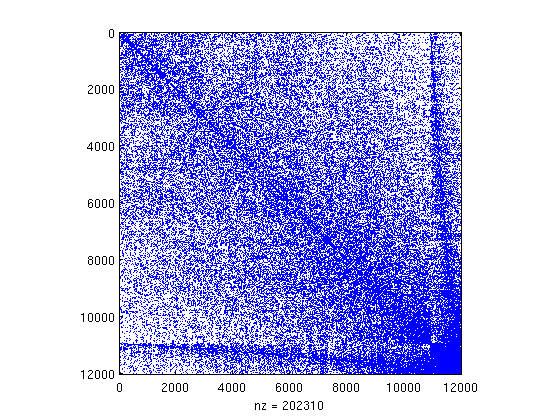
\includegraphics[scale=0.65]{spyAA}
    \caption{Sparsity pattern of $\widehat{A}$}
    \label{spyAA}
  \end{figure}
\item
  We can now resolve the generalized eigen problem with $\widehat{A}$ and $\widehat{B}$.
\item
  Finally, to retrieve the original eigen functions, we need to multiply the eigen functions by $C$.
  \lstinputlisting[widthgobble=2*2,linerange=eigenvec]{../../src/basischange.cpp}
\end{itemize}

\subsection{Timing}

The figure \ref{timeC} shows the time take to accomplish the steps for creating the matrix $C$. \texttt{indexes} corresponds to the steps for retrieving the informations on the dofs and the indexes to keep in the matrix. \texttt{fill} corresponds to the steps of creating the two matrices, fill them and assembling them. \texttt{submatrix} corresponds to sorting the vector of indexes, and removing the columns to have $C$. These tests have been conducted on the cylinder.\\

\begin{figure}[H]
  \centering
  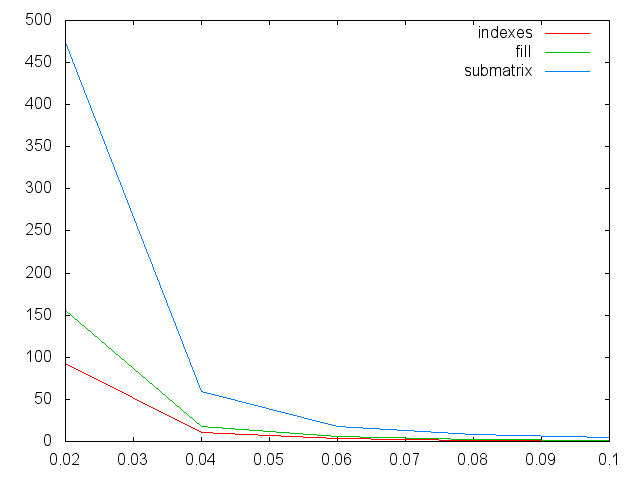
\includegraphics[scale=0.7]{createC}
  \caption{Time to compute C}
  \label{timeC}
\end{figure}

We could think that the time increase really fast but the figure \ref{completeTime} shows the percentage of the total time take for the steps. \texttt{mesh} corresponds to the loading of the mesh, \texttt{space} create $\NN_h$ and $\LLL_h$, and \texttt{forms} create the matrix $A$ and $B$.\\
We see that in fact the percentage of time is constant for each steps.

\begin{figure}[H]
  \centering
  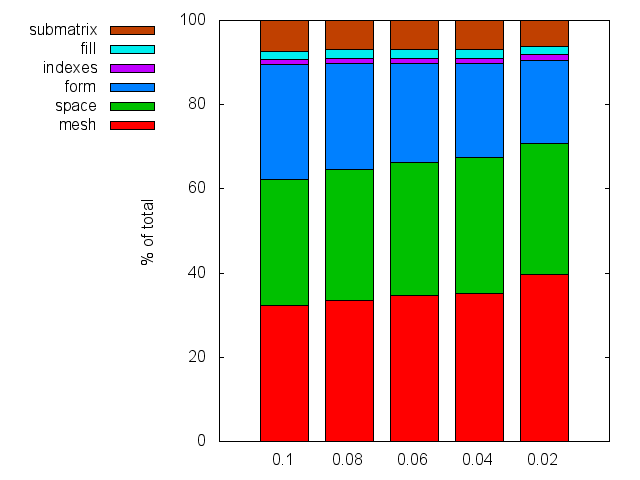
\includegraphics[scale=0.7]{completeChBase}
  \caption{Time to compute the changement of basis}
  \label{completeTime}
\end{figure}

For an idea, we have the following number of dofs depending on the size of the mesh for the cylinder :
\begin{center}
  \begin{tabular}{ c | c | c | c }
    $h$ & \#dof($\NN_h$) & \#dof($\LLL_h$) & \#columns of $C$ \\ \hline
    0.1 & 23\,943 & 3\,908 & 19\,867 \\ \hline
    0.08 & 48\,016 & 7\,593 & 41\,322 \\ \hline
    0.06 & 107\,447 & 16\,414 & 95\,669 \\ \hline
    0.04 & 333\,704 & 49\,202 & 308\,086 \\ \hline
    0.02 & 2\,598\,692 & 367\,288 & 2\,497\,232 \\ \hline
  \end{tabular}
\end{center}

\section{Results}

I find the 6 first eigenvalue in the sphere, using the following configuration :
\begin{description}
\item[solver] krylovschur
\item[problem] ghep
\item[transform] shift\_invert
\item[spectrum] smallest\_magnitude
\item[target] 15
\end{description}

The figure \ref{feelModes} presents the first mode for the sphere and for the rectangular box.
\begin{figure}[H]
  \makebox[\textwidth][c]{
    \subfloat[Sphere]{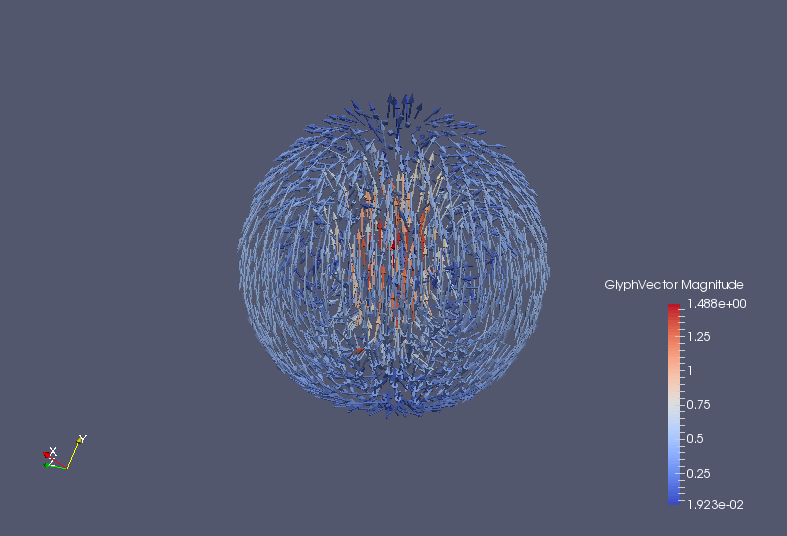
\includegraphics[scale=0.27]{sphMode0}}\ 
    \subfloat[Rectangular Box]{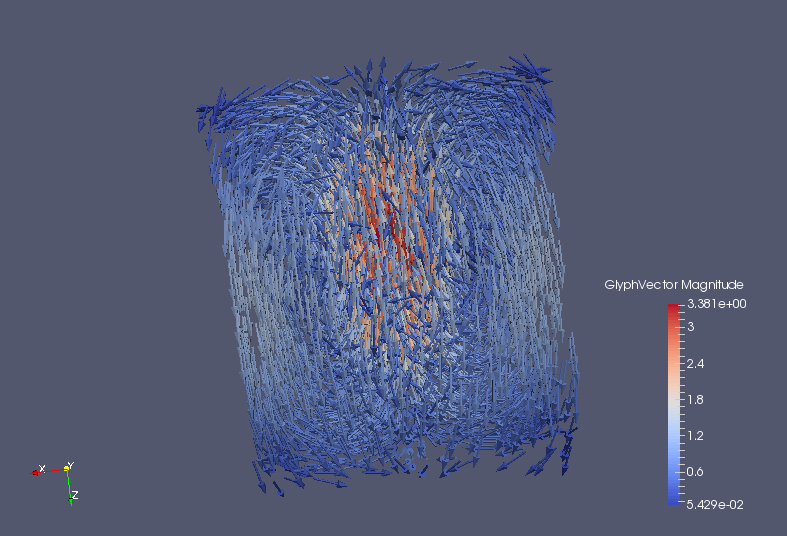
\includegraphics[scale=0.27]{rbMode0}}
  }
  \caption{Eigen Functions from Feel++}
  \label{feelModes}
\end{figure}

To understand the link between those functions and the eigen functions of the curl operator, I'll quote the article \cite{Venegas2013} :
\begin{italicquotes}
  According to the theoretical results, the invariant subspace spanned by the six eigenfunctions of Problem \ref{pbdiscr} corresponding to $\lambda_{h,1},\dots,\lambda_{h,6}$ yields an approximation of the eigenspace of $\lambda^2$ in Problem \ref{pbweak}. However, the latter is the direct sum of two three-dimensional eigenspaces of Problem \ref{pbstart}, those corresponding to $\lambda$ and $-\lambda$. Therefore, the eigenfunctions of Problem \ref{pbdiscr} are not in general eigenfunctions of Problem \ref{pbstart} (and hence Beltrami fields), but a linear combination of eigenfunctions corresponding to both eigenvalues, $\lambda$ and $-\lambda$.
\end{italicquotes}
It means that if we have $(\lambda^2,\mbf{u}_i)$ solutions of Problem \ref{pbdiscr}, and $(\pm\lambda,\mbf{v}_i)_{i=1,\dots,m}$ solutions of Problem \ref{pbstart}, we have : $\mbf{u}_i=\sum_{j=1}^m \beta_j\mbf{v}_i$.\\

And indeed, we do not have that $\curl\mbf{u}_i-\lambda_i\mbf{u}_i = 0$.\\
For the first eigenvalue, we have the following results :
\begin{table}[H]
  \centering
  \begin{tabular}{r|c|c|c}
    h & 0.15 & 0.075 & 0.05 \\
    \# elements & 7000 & 50000 & 150000 \\
    \hline
    $\widehat{\lambda}_h$ & 4.49481924 & 4.49377347 & 4.49361\\
    $|\widehat{\lambda}_h-\lambda|$ & 0.00141024 & 0.00036447 & 0.000201 \\
    order & $-$ & 1.9521 & 1.4678 \\
    \hline
    $||\div\mbf{u}||_2$ & 2.88311e-14 & 6.60701e-14 & 9.22039e-14 \\
    $||\mbf{u}\cdot\mbf{n}||_2$ & 0.216208 & 0.112487 & 0.0737108 \\
    $||\curl\mbf{u}\cdot\mbf{n}||_2$ & 5.11927e-15 & 9.48309e-15 & 1.47194e-14 \\
    $||\curl\mbf{u}-\lambda\mbf{u}||_2$ & 6.5155 & 6.38584 & 6.381
  \end{tabular}
  \caption{Results in the sphere}
\end{table}
where $\widehat{\lambda}_h=\sum_{i=1}^6\lambda_{i,h}/6$
\begin{rk}\label{curll}
  To check if $\curll\mbf{u}=\lambda^2\mbf{u}$, we can solve two systems :
  \begin{itemize}
  \item $-\laplace\mbf{x}=\lambda^2\mbf{u}$
  \item $\curll\mbf{u}=\lambda^2\mbf{u}$
  \end{itemize}
  and check if $\mbf{x}=\mbf{u}$, but in the first case, the boundary conditions are not set correctly, and in the second case, the solver doesn't converge, certainly because we are not in the space $\ZZ_h$ but in $\NN_h$.
\end{rk}

\begin{table}[H]
  \centering
  \begin{tabular}{c|cc|c|c}
    h & 0.075 & 0.05 & exact & order \\
    \# elements & 10000 & 35000 & - & - \\
    \hline
    $\widehat{\lambda}_{h,1}$ & 7.42151 & 7.42658 & 7.4319 & 1.6509 \\
    $\widehat{\lambda}_{h,2}$ & 7.76569 & 7.77023 & 7.7763 & 1.3773 \\
    $\widehat{\lambda}_{h,3}$ & 8.07633 &  8.08247 & 8.0909 & 1.3495
  \end{tabular}
  \caption{Results in the rectangular box}
\end{table}

We can see that the divergence and the normal component of the curl are zero, but the normal component of the function is not exactly zero, but tends to dicrease as $h$ tends to 0.\\
The important thing is that the eigenspaces are equivalents.\\



%%% Local Variables:
%%% TeX-master: "../peps.tex"
%%% eval: (flyspell-mode 1)
%%% ispell-local-dictionary: "english"
%%% End:
